\documentclass[aps,prb,onecolumn,nofootinbib,superscriptaddress]{revtex4-2}
\usepackage{amsmath,amssymb,amsthm,mathtools,bm}
\usepackage{booktabs}
\usepackage{graphicx}
\usepackage[colorlinks=true,linkcolor=blue,citecolor=blue,urlcolor=blue]{hyperref}
\usepackage{microtype}

\newcommand{\Tr}{\operatorname{Tr}}
\newcommand{\E}{\mathbb{E}}
\newcommand{\med}{\operatorname{med}}
\newcommand{\se}{\operatorname{SE}}

\begin{document}

\title{What the CPU CFT-Extraction Experiments Actually Establish}
\author{Asadullah Bhuiyan}
\noaffiliation
\date{August 15, 2026}

\begin{abstract}
This note audits the completed CPU experiments in \texttt{cpu\_cft\_extraction} from the
formal target through the numerical implementation, saved arrays, fits, figures, and
convergence diagnostics.  The calculation sought the effective central charge from the
finite-size correction to a trajectory free-energy density and typical scaling dimensions
from tangent-cocycle and Choi-transfer gaps.  The pipeline successfully measures a slow
interface channel and, at moderate time, the two independent Gaussian spectral routes give
a mutually consistent candidate scale near $x\simeq0.19$.  The experiments do \emph{not}
yet determine $c_{\rm eff}$ or an asymptotic scaling dimension.  The fitted central charge
changes from $-345$ at $T/L=2$ to $-159$ at $T/L=5$ and $+40$ at $T/L=20$, while the
underlying free-energy curves retain measurable temporal drift.  At $T/L=20$ the Choi
eigenvalues have saturated to the numerical endpoints $\pm1$, eliminating every final-time
finite rapidity.  The remaining long-time tangent estimate is strongly dependent on whether
the finite-size fit is allowed a nonzero intercept.  These are convergence and numerical
dynamic-range failures, not evidence for the large quoted central charges.  The main
positive outcome is therefore methodological: the observable pipeline works and exposes a
structured low-lying transfer spectrum, but a controlled CFT extraction requires seeded
reproducibility, late-time increment estimators, higher statistics, sector-resolved gaps,
and a log-stable Choi formulation.
\end{abstract}

\maketitle
\setcounter{tocdepth}{2}
\tableofcontents

\section{Scope and bottom line}

The evidentiary boundary is deliberately conservative.  This note uses only campaigns for
which the driver wrote the complete scalar table and all per-size trajectory, tangent, and
Choi files.  It includes
\begin{enumerate}
\item $N_x=20$, $L=N_y=20,30,40$, $T=2L$, ten samples per size;
\item $N_x=20$, $L=20,30,40$, $T=5L$, ten samples per size, formed by combining the
separately completed $L=20$ and $L=30,40$ runs with identical declared parameters; and
\item $N_x=20$, $L=20,22,24$, $T=20L$, ten samples per size.
\end{enumerate}
The $T=20L$, $L=26,28,30$ extension was still running when this note was prepared.  It is
not used in a fit, table, trend, or extrapolation.  In particular, the completed $T=5L$ and
the unfinished $T=20L$ realizations at $L=30$ are never mixed.

The conclusions, ordered from strongest to weakest, are:
\begin{enumerate}
\item The implemented experiment detects a slow, size-dependent interface transfer mode.
The tangent and Choi routes track one another closely while both are numerically resolved.
\item At $T/L=5$, direct and through-origin gap estimates from both routes cluster near
$x\simeq0.19$.  This is a useful preasymptotic candidate, not a measured universal exponent.
\item The central-charge extraction is uncontrolled.  Its sign and magnitude change with
the run time, and the expected $O(L^{-2})$ signal is much smaller than the present statistical
and temporal systematics.
\item The late-time Choi failure is understood: finite rapidities are exponentially mapped
to eigenvalues indistinguishable from $\pm1$ under the fixed endpoint tolerance.  Endpoint
counts consequently mix physical endpoint modes with finite-precision saturation.
\item The rank scan reveals a smooth additive low-energy tower and striking tangent--Choi
agreement through the range where the Choi data remain supported.  Since it is a
postprocessing sum of one-body order statistics at $T/L=2$, it is not yet a sector-resolved
CFT spectrum.
\end{enumerate}

\section{Formal target}

\subsection{Trajectory weights and the cylinder free energy}

For a measurement record $\xi=(m_1,\ldots,m_t)$ sampled with the Born rule, the normalized
trajectory probability is
\begin{equation}
 p_\xi=\prod_{k=1}^{t}p(m_k\mid m_1,\ldots,m_{k-1}),
 \qquad Y_\xi=-\log p_\xi.
\end{equation}
The code accumulates exactly this $Y_\xi$ for the physical measurement sequence used here;
the perfect-correction factor is unity, so its logarithm vanishes.  With circumference $L$
and the conversion between circuit cycles and isotropic Euclidean time denoted by $\alpha$,
the finite-time estimator is
\begin{equation}
 f_0(L,t)=\frac{1}{\alpha L t}\E_\xi[Y_\xi(t)].
 \label{eq:f0}
\end{equation}
If the long-distance replicated transfer problem is governed by a conformal fixed point on
a cylinder, its stationary free-energy density has the expansion
\begin{equation}
 f_0(L)=f_\infty-\frac{\pi c_{\mathrm{eff}}}{6L^2}
 +\frac{b_4}{L^4}+\cdots .
 \label{eq:ceff}
\end{equation}
Thus a straight-line fit of $f_0$ versus $L^{-2}$ has slope
$-\pi c_{\mathrm{eff}}/6$.  This statement presupposes the limits $t/L\to\infty$ and
$L\to\infty$, a fixed and calibrated $\alpha$, and sufficiently small irrelevant and
boundary corrections.  A numerically precise line through three transient points is not by
itself evidence that these conditions hold.

There is also an estimator issue worth separating from physics.  The production output uses
the cumulative value in Eq.~\eqref{eq:f0} at the final cycle.  If initialization contributes
an $O(L)$ boundary term $B_\xi$, then
\begin{equation}
 \frac{Y_\xi(t)}{Lt}=f_0(L)+\frac{B_\xi}{Lt}+\cdots,
\end{equation}
so convergence is only algebraic in time.  A late-time slope of $Y_\xi/L$, or block
increments $[Y(t_2)-Y(t_1)]/[L(t_2-t_1)]$, removes the leading additive boundary term and is
the more appropriate stationary estimator.

\subsection{Typical transfer gaps and scaling dimensions}

Let $S_A(\xi,t)$ denote a singular value or sector amplitude of the trajectory transfer
operator, with $S_0$ the dominant reference.  The quenched or typical gap is formally
\begin{equation}
 \mu_A=-\lim_{t\to\infty}\frac{1}{t}
 \E_\xi\log\left|\frac{S_A(\xi,t)}{S_0(\xi,t)}\right|.
 \label{eq:quenchedgap}
\end{equation}
At a conformal fixed point,
\begin{equation}
 \mu_A(L)=\frac{2\pi\alpha}{L}x_A^{\mathrm{typ}}+o(L^{-1}),
 \qquad
 \frac{\mu_A(L)}{\alpha L}=\frac{2\pi x_A^{\mathrm{typ}}}{L^2}+\cdots .
 \label{eq:xfit}
\end{equation}
The production fit therefore regresses $\mu/(\alpha L)$ against $L^{-2}$ and divides the
slope by $2\pi$.  Allowing a free intercept is a diagnostic for corrections or a residual
noncritical gap.  With only three nearby sizes, however, slope and intercept can trade
strongly; a through-origin fit provides an important sensitivity check rather than an
alternative theorem.

The formal quenched average in Eq.~\eqref{eq:quenchedgap} is a mean of trajectory logarithms.
The scripts instead take the median of the per-trajectory smallest finite rates and
bootstrap that median.  This robust statistic is sensible in a heavy-tailed sample of ten,
but it is not exactly the formal estimator.  The distinction must remain explicit until
the mean, median, and tail behavior are compared at substantially higher statistics.

\subsection{Tangent cocycle}

Linearizing the Gaussian covariance update about a physical trajectory defines a random
tangent cocycle.  QR stabilization accumulates logarithmic stretch factors and produces
finite-time Lyapunov rates $\lambda_j(t)$.  The implemented one-body proxy is
\begin{equation}
 \Delta_{\mathrm{tan}}(t)=\min_j|\lambda_j(t)|.
 \label{eq:tangap}
\end{equation}
Interpreting Eq.~\eqref{eq:tangap} as a CFT transfer gap assumes that the neutral or dominant
reference exponent is exactly zero and that the corresponding one-quasiparticle excitation
is permitted in the target sector.  More generally the physical quantity is a difference
$|\lambda_j-\lambda_0|$ with charge and parity constraints.  The QR code also clips null
directions to large finite negative logarithms; the saved null count is cumulative over QR
events, not the multiplicity of final modes removed from a spectrum.

\subsection{Choi/Kraus transfer spectrum}

The second construction contracts the cumulative Gaussian channel into a reduced Choi
covariance.  Its canonical eigenvalues occur as $\pm a_j$ with $|a_j|\leq1$.  Finite
single-particle rapidities are reconstructed as
\begin{equation}
 \epsilon_j(t)=\frac{|\operatorname{artanh}a_j(t)|}{t},
 \qquad
 \Delta_{\mathrm{Choi}}(t)=\min_j\epsilon_j(t).
 \label{eq:choigap}
\end{equation}
The implementation calls $a_j$ an endpoint when
$\bigl||a_j|-1\bigr|<10^{-8}$ and excludes it from Eq.~\eqref{eq:choigap}.  This is necessary
for exact gain/loss null sectors, but a finite rapidity also obeys
$a_j=\tanh(t\epsilon_j)$ and therefore approaches an endpoint exponentially.  The fixed
tolerance implies an approximate dynamic-range ceiling
\begin{equation}
 \epsilon_{\max}^{\mathrm{resolvable}}(t)
 \simeq \frac{\operatorname{artanh}(1-10^{-8})}{t}
 \simeq \frac{9.56}{t}.
 \label{eq:dynamicrange}
\end{equation}
Going to longer time can therefore make this estimator \emph{less} informative in ordinary
double precision.

The tangent and Choi calculations are different transfer objects; no exact identity between
their finite-time spectra is assumed.  Agreement is valuable cross-validation that the two
constructions see a common slow mode.  Disagreement can arise from finite time, numerical
conditioning, or genuinely distinct sector content.

\subsection{What ``Fock rank'' means in these files}

For a free-fermion transfer problem, a many-body excitation can be an allowed sum of
single-particle rapidities.  The postprocessor defines a rank-$R$ proxy by summing the $R$
smallest positive magnitudes.  Every completed production campaign was run with
\texttt{fock\_rank=1}; consequently the saved ``Fock'' gap is exactly the one-body proxy.
The ranks $R=2,\ldots,10$ were generated later from the same $T/L=2$ spectra.  No separate
fixed-charge, parity, particle--hole, or operator-sector transfer calculation was performed.

\section{What was simulated}

\subsection{Geometry and circuit protocol}

All production data use $N_x=20$ and periodic length $N_y=L$.  The domain-wall slab contains
the columns $x=4,\ldots,16$, thirteen columns in total, so the reduced one-body dimension is
$2\times13L=26L$.  The CPU class is configured with a domain wall, one shell,
$\alpha_1=1$, $\alpha_2=30$, and domain-wall truncation.  The initial state is a random pure
half-filled Gaussian covariance; the exterior is projected once into an onsite product
state.

Each cycle visits the active slab in \texttt{raster\_y} order.  At each site the four
measurement channels $A_+,A_-,B_+,B_-$ are sampled by their Born probabilities.  The upper
and lower targets are respectively empty and occupied.  The campaigns have no forced
postselection and use perfect correction, so the accumulated record weight is the product
of measurement Born probabilities.  Tangent, Choi, and trajectory-weight observers are
attached to the same canonical call to
\texttt{classA\_U1FGTN.run\_markov\_circuit}; parallelism is across independent one-sample
workers, with one BLAS thread per worker.

The analysis sets $\alpha=1$.  This is an anisotropy convention in
Eqs.~\eqref{eq:f0}--\eqref{eq:xfit}, not the mass parameter $\alpha_1$.  No independent
velocity or aspect-ratio calibration was performed, so any quoted $c_{\rm eff}$ or $x$ is
conditional on this convention.

\subsection{Saved estimators and uncertainty convention}

For each size the production script saves the final cumulative mean of $Y/(\alpha Lt)$ and a
512-resample trajectory bootstrap standard error.  It saves the median smallest finite
tangent and Choi rate and a corresponding bootstrap standard error.  The campaign fit is an
unweighted two-parameter least-squares fit to the central values.  Its reported slope error
comes only from the residual scatter of two or three points and does not propagate the
per-size bootstrap errors.  Throughout this note those tiny three-point errors are described
as regression diagnostics, not as full physical uncertainties.  Weighted fits using the
saved per-size errors and through-origin fits are quoted as sensitivity tests.

There is no burn-in: tangent rates and the cumulative free energy begin at the first cycle.
The convergence diagnostic used below compares the mean value over the final quarter of the
time series with the mean over the preceding quarter,
\begin{equation}
 \delta_Q=100\left(\frac{\overline O_{[3T/4,T]}}
 {\overline O_{[T/2,3T/4]}}-1\right)\% .
\end{equation}

\subsection{Campaign ledger}

\begin{table}[b]
\caption{Completed production campaigns used in this note.  Each size contains ten
trajectories.}
\label{tab:ledger}
\begin{ruledtabular}
\begin{tabular}{lcccc}
label & $L$ & cycles $T$ & $T/L$ & role \\
\hline
short & $20,30,40$ & $40,60,80$ & 2 & pipeline and rank scan \\
moderate & $20,30,40$ & $100,150,200$ & 5 & best tangent--Choi overlap \\
long & $20,22,24$ & $400,440,480$ & 20 & temporal convergence stress test \\
\end{tabular}
\end{ruledtabular}
\end{table}

\section{Numerical results}

\subsection{Free energy and effective central charge}

The central result is instability, not a central charge.  Table~\ref{tab:ceff} lists the
free-intercept fits used by the repository and weighted sensitivity fits.  Increasing
$T/L$ changes both sign and magnitude of the result.  The $T/L=20$ sizes also span only
$20\leq L\leq24$, making the intercept and $L^{-2}$ slope particularly covariant.

\begin{table}[t]
\caption{Central-charge fits from completed campaigns.  ``OLS diagnostic'' is the saved
unweighted three-point regression error; ``WLS sensitivity'' propagates the saved per-size
standard errors but still does not include temporal or window systematics.}
\label{tab:ceff}
\begin{ruledtabular}
\begin{tabular}{cccc}
$T/L$ & sizes & $c_{\mathrm{eff}}$ (OLS diagnostic) & $c_{\mathrm{eff}}$ (WLS sensitivity) \\
\hline
2  & $20,30,40$ & $-345.17\pm21.48$ & $-347.85\pm35.16$ \\
5  & $20,30,40$ & $-158.55\pm25.38$ & $-165.45\pm29.83$ \\
20 & $20,22,24$ & $+40.16\pm15.02$  & $+45.29\pm34.98$ \\
\end{tabular}
\end{ruledtabular}
\end{table}

\begin{figure}[t]
\centering
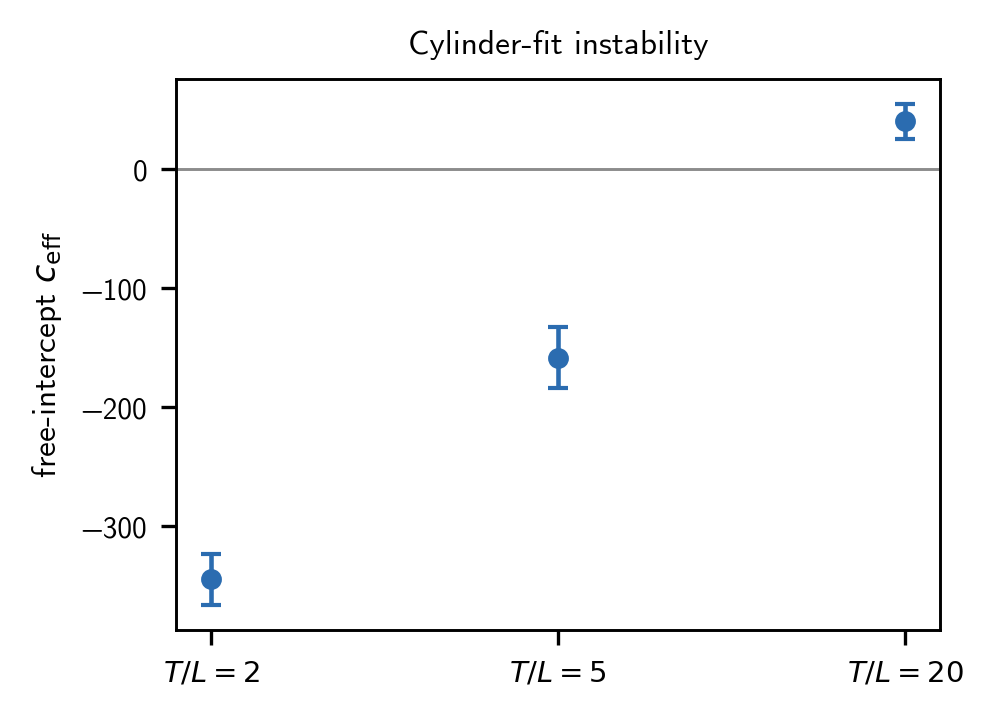
\includegraphics[width=3.375in]{figures/central_charge_stability.png}
\caption{The nominal cylinder-fit central charge is not stable under increasing $T/L$.
Bars show only the unweighted three-point regression diagnostic.}
\label{fig:ceff}
\end{figure}

The free-energy quarter drifts are $(-7.65,-5.71,-4.45)\%$ at $T/L=2$,
$(-3.61,-2.80,-2.18)\%$ at $T/L=5$, and $(-0.80,-0.91,-1.01)\%$ at $T/L=20$ in ascending
$L$.  The longer run is visibly better, but a one-percent temporal bias is still large
compared with the desired cylinder correction.  For orientation, a $c=1$ signal changes
$f_0$ by only about $4\times10^{-4}$ between $L=20$ and $L=24$, whereas the standard error
of their observed difference is about $1.4\times10^{-2}$.  Ten trajectories are therefore
underpowered for a unit-order central charge even before accounting for drift.

As an explicit estimator sensitivity check, fitting the slope of $Y/L$ over the final half
of each $T/L=20$ trajectory gives stationary-rate estimates approximately
$3.170\pm0.019$, $3.171\pm0.021$, and $3.175\pm0.008$ for $L=20,22,24$.  Their weighted
cylinder fit yields $c_{\rm eff}=13\pm50$.  This supports a bulk Born free-energy rate near
$3.17$ and, correctly, no useful central-charge determination.

\subsection{Gap and scaling-dimension estimates}

The direct size estimator
\begin{equation}
 x_{\mathrm{dir}}(L)=\frac{L\Delta(L)}{2\pi\alpha}
\end{equation}
is the least extrapolation-dependent view of the gap data.  Figure~\ref{fig:directx} shows
that the $T/L=5$ tangent and Choi points lie near one another and near $0.19$, whereas the
long tangent values fall across $0.281$, $0.276$, and $0.237$.  The latter trend is not a
stable plateau.

\begin{figure}[t]
\centering
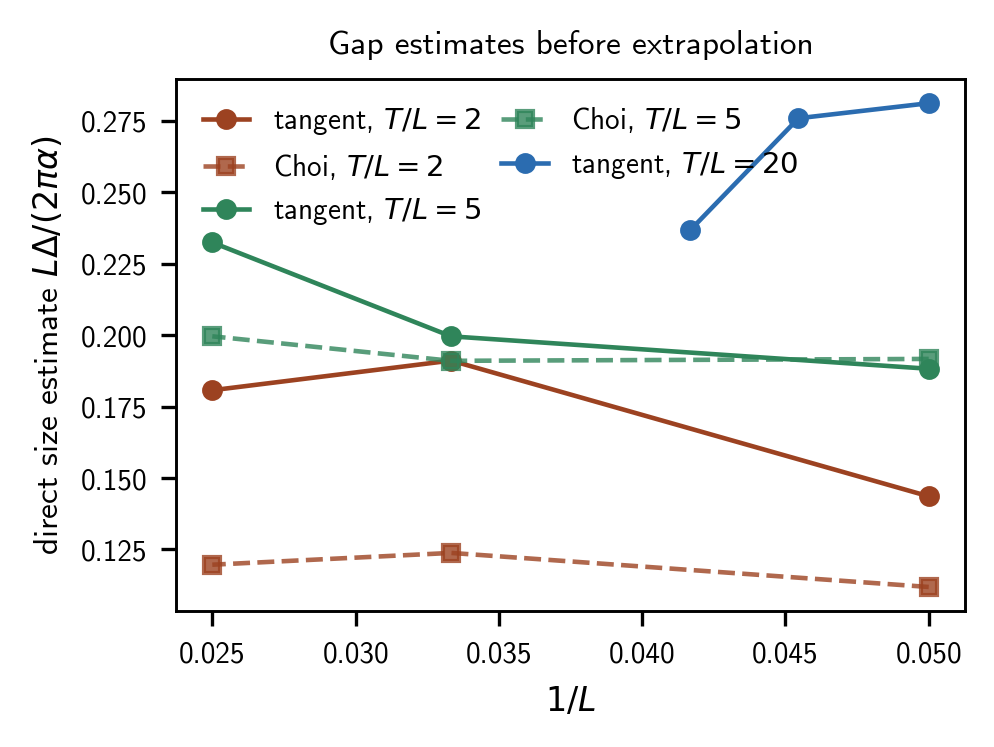
\includegraphics[width=3.375in]{figures/direct_gap_estimates.png}
\caption{Direct, per-size scaling estimates.  These make visible the finite-time evolution
that is hidden by a single extrapolated headline.  No Choi point exists at the final time of
the $T/L=20$ run.}
\label{fig:directx}
\end{figure}

\begin{table}[t]
\caption{Scaling-dimension fit sensitivity.  The free-intercept uncertainty is only the
three-point regression diagnostic; the WLS uncertainty uses saved gap errors.}
\label{tab:xfit}
\begin{ruledtabular}
\begin{tabular}{ccccc}
$T/L$ & route & free-intercept $x$ & WLS $x$ & through-origin $x$ \\
\hline
2 & tangent & $0.1256\pm0.0203$ & $0.1556\pm0.0435$ & $0.1529$ \\
2 & Choi    & $0.10775\pm0.00551$ & $0.1130\pm0.0388$ & $0.1141$ \\
5 & tangent & $0.17475\pm0.00450$ & $0.1676\pm0.0321$ & $0.1922$ \\
5 & Choi    & $0.18974\pm0.00251$ & $0.1863\pm0.0281$ & $0.1920$ \\
20 & tangent & $0.3785\pm0.0496$ & $0.3645\pm0.0199$ & $0.2696$ \\
20 & Choi & \multicolumn{3}{c}{no finite final-time rapidity} \\
\end{tabular}
\end{ruledtabular}
\end{table}

The moderate-time result is the most internally coherent spectral observation.  The Choi
free-intercept is $2.60\times10^{-5}$, consistent with zero at the three-point regression
level, and both through-origin routes yield $x\simeq0.192$.  However, the tangent intercept
is $2.04\times10^{-4}$, the final-quarter drifts are still $(18.2,15.8,-3.0)\%$ for tangent
and $(31.4,12.7,6.3)\%$ for Choi, and the per-size uncertainties broaden the two values to
$0.168\pm0.032$ and $0.186\pm0.028$.  The correct statement is therefore that
$x\approx0.19$ is a cross-validated finite-time candidate.

The long tangent free-intercept fit illustrates the danger of extrapolating three narrow
sizes: it gives $x=0.3785$ while its fitted intercept is
$-1.47(66)\times10^{-3}$.  A through-origin fit gives $0.2696$, close to the mean of the
three direct estimates, $0.2646$.  This $40\%$ shift is much larger than the displayed
regression error.  The long tangent quarter drifts remain $2.1$--$3.3\%$.  It is premature
to decide whether the asymptotic value is near $0.19$, near $0.25$, or elsewhere.

\subsection{Why the long-time Choi gaps disappear}

At $T/L=20$ the final reduced Choi dimension is entirely classified as endpoint:
$520$, $572$, and $624$ modes for $L=20,22,24$.  Every one of the ten samples at every size
has a nonfinite final Choi gap.  The last cycles at which \emph{any} sample retains a finite
gap are $161$, $191$, and $259$, corresponding to $t/L\simeq8.05$, $8.68$, and $10.79$.
Across the full histories only $1294/4000$, $1511/4400$, and $1846/4800$ sample-cycle gaps
are finite.

\begin{figure}[t]
\centering
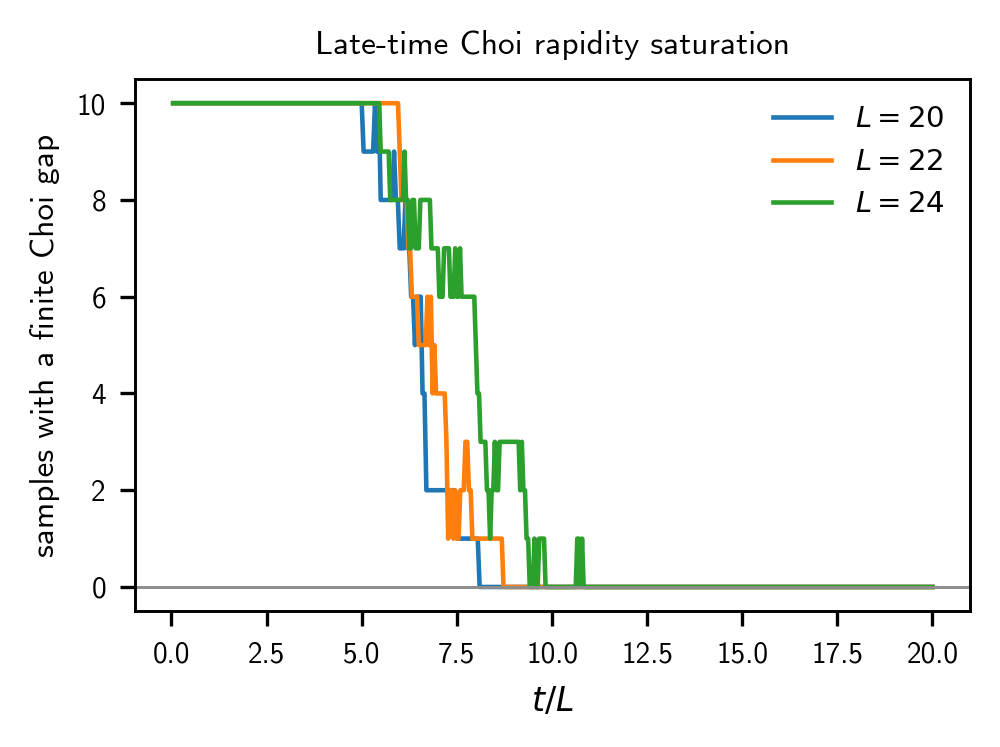
\includegraphics[width=3.375in]{figures/choi_saturation.png}
\caption{Number of samples, out of ten, with a finite Choi gap during the completed
$T/L=20$ campaign.  Finite rapidities are eventually mapped inside the fixed $10^{-8}$
endpoint tolerance and disappear.}
\label{fig:choisaturation}
\end{figure}

The saved endpoint flag is therefore a finite-precision statement at long time, not a count
of exact null sectors.  Moreover, \texttt{choi\_censored\_count=0} does not contradict the
failure: the ``censor'' branch regularizes small denominators without deactivating the
sample, the recorder leaves the active flag unchanged, and final aggregation does not use
that flag to filter gaps.  The final Choi eigenvalues lie within roughly $10^{-11}$ of the
endpoints, far inside the $10^{-8}$ threshold.  Shorter-time Choi gaps should consequently
be treated as finite-time, finite-dynamic-range estimates, not a demonstrably converged
limit.

\subsection{Additive rank scan}

The $T/L=2$ postprocessing scan gives tangent/Choi pairs
\begin{equation}
 (x_1,\ldots,x_5)_{\rm tan}=(0.126,0.343,0.684,1.246,1.935),
\end{equation}
and
\begin{equation}
 (x_1,\ldots,x_5)_{\rm Choi}=(0.108,0.356,0.713,1.230,1.937).
\end{equation}
The agreement for ranks $2$--$5$ is at the few-percent level.  Choi support then collapses:
rank five has only $7,7,8$ valid samples across the sizes, rank six has $3,0,3$, and higher
ranks have none.  The tangent construction continues through rank ten.

\begin{figure}[t]
\centering
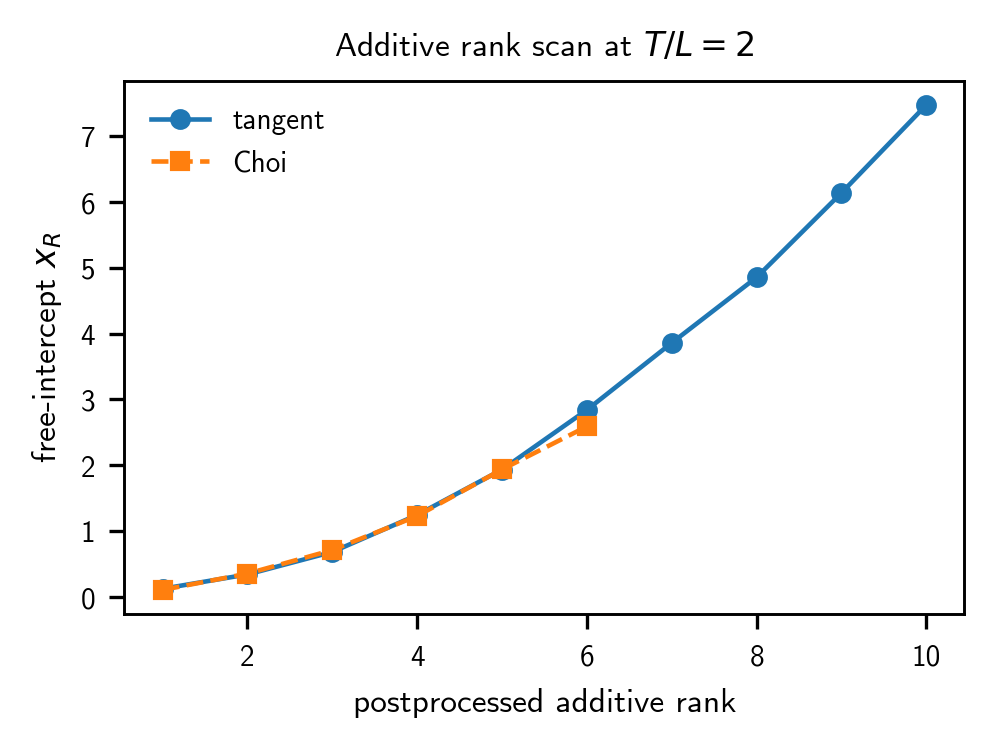
\includegraphics[width=3.375in]{figures/rank_scan_comparison.png}
\caption{Free-intercept fits to additive sums of the $R$ smallest one-body rates at
$T/L=2$.  The smooth, convex sequence is a real structural observation, but it is neither
an independently simulated many-body tower nor sector resolved.}
\label{fig:rankscan}
\end{figure}

This is strong evidence that both Gaussian routes order the same low-lying one-body content
before Choi saturation.  It is not evidence for particular CFT primaries: additive order
statistics automatically produce a smooth convex tower, and the short-time spectra are the
least converged data in the campaign.

\section{Implementation and provenance audit}

\subsection{Reproducibility hole}

The driver hashes the declared seed and sample index, calls
\texttt{numpy.random.seed(seed)}, and records the rule in the manifest.  It does not pass
that seed as \texttt{random\_seed} to \texttt{run\_markov\_circuit}.  The default initial
state inside the engine uses a new \texttt{numpy.random.default\_rng()} seeded from entropy.
Thus the measurement draws may follow the legacy global seed while the initial random pure
covariance does not.  Repeating the same declared sample does not reproduce the full
trajectory, and nominally overlapping short and long runs are not exact prefixes.

This does not invalidate the saved samples as stochastic draws, but it prevents paired
finite-time comparisons and makes the manifest's seed rule incomplete.  It also means that
the separately completed $T/L=5$ sizes can be combined only as independent samples under a
common declared ensemble, not as a prefix-coupled dataset.

\subsection{Manifest completeness and code state}

The manifests record the repository commit and principal sweep flags but omit fixed settings
needed to reconstruct the ensemble: domain-wall activation, shell count, mass parameters,
truncation, initialization mode and filling, site sequence, active-slab restriction, and the
physical-update convention.  In addition, the extraction directory was untracked and the
engine had local modifications, so the recorded commit alone does not pin the executed code.
The long live process also loaded its Python source before a later source-file modification.
Future manifests should record a source-tree diff or content hashes for the driver and engine,
plus the complete resolved configuration.

\subsection{What the tests establish}

The local suite contains eight passing checks covering synthetic fit algebra, endpoint
classification, gap helpers, observer plumbing, refusal of postselection, parallel output
shapes, and a small benchmark.  The tangent primitive has additional cocycle tests elsewhere
in the repository.  These checks establish that the pipeline is wired together and that the
saved quantities follow the intended elementary formulas.

They do not test finite-time convergence, full seed reproducibility, late Choi saturation,
regularization bookkeeping, inactive-sample filtering, tangent null masking, a nontrivial
Fock sector, or an exactly solvable tangent--Choi spectral comparison.  Scientific
convergence therefore cannot be inferred from unit-test success.

\section{Interpretation}

\subsection{What is supported}

The most defensible physical statement is that this interface circuit has a slow transfer
channel whose finite-time rate scales roughly as $1/L$ over the simulated window.  Two
substantially different Gaussian diagnostics identify the same channel at moderate time,
their trajectory-level values are strongly correlated, and their additive low-lying order
statistics agree before the Choi representation runs out of precision.  These facts make it
unlikely that the entire signal is a plotting or indexing artifact.

A second supported statement is that the stationary bulk Born free-energy density is near
$3.17$ in the long runs.  Its small residual size dependence is presently statistically
consistent with many values of $c_{\rm eff}$, including an ordinary order-one value.

\subsection{What is not supported}

The experiments do not support a numerical value or even a stable sign for
$c_{\rm eff}$.  The large negative short-time fits should not be called exotic central
charges; they follow the same direction as the explicit temporal drift and change radically
with run length.  Nor do the experiments select a final $x^{\rm typ}$.  The value near
$0.19$ is the best cross-route finite-time candidate, while the longer tangent data suggest
a larger direct scale but fail the extrapolation-stability test.  The Choi route cannot
arbitrate because it has saturated.

The endpoint count is not a universal observable in its current form.  It is dominated by
the extensive reduced dimension and, at long time, by tolerance-dependent numerical
saturation.  The rank scan is not a conformal tower assignment because sector selection is
absent.  Finally, the present data cannot test whether $\alpha=1$ is the isotropic CFT
normalization.

\subsection{Overall take}

These experiments are a successful stress test of the proposed extraction strategy and a
failed asymptotic measurement.  That distinction is useful.  The data identify precisely
where the naive program breaks: cumulative free energies converge too slowly to resolve an
$L^{-2}$ Casimir term at ten samples; free-intercept gap fits are fragile over three sizes;
and the direct Choi parametrization loses exponential information at the times needed for
Lyapunov convergence.  The correct next step is not to quote a compromise number from the
existing fits, but to redesign the estimators around those failure modes.

\section{Recommended next numerical program}

\begin{enumerate}
\item \textbf{Repair reproducibility first.}  Pass the resolved sample seed directly to the
canonical engine, record it, and test bitwise prefix equality across run lengths and worker
counts.  Save content hashes for all executed sources and the fully resolved model settings.

\item \textbf{Separate the cheap free-energy campaign.}  Run a Born-weight-only ensemble
with many more trajectories and more sizes.  Estimate $f_0(L)$ from late-time slopes or
blocked increments, scan the fit window, and use a nested trajectory bootstrap for the
finite-size fit.  Compare $L^{-2}$ and $L^{-2}+L^{-4}$ models.  Suppress a central-charge
headline unless temporal drift is below the targeted Casimir signal.

\item \textbf{Use stationary tangent windows.}  Introduce a burn-in, accumulate QR rates in
late windows, and verify window stability.  Report direct $L\Delta/(2\pi\alpha)$ points,
free-intercept fits, and through-origin fits together.  Increase the $L$ range before
interpreting a fitted intercept.

\item \textbf{Reformulate the Choi extraction.}  Carry logarithmic singular values or a
QR/SVD product representation rather than recovering rapidities from $a=\tanh(t\epsilon)$
near $|a|=1$.  At minimum save finite-mode counts, last finite cycle, denominator
regularization records, and tolerance scans.  A precision and endpoint-tolerance study is a
required validation, not an optional cosmetic check.

\item \textbf{Define physical sectors.}  Construct allowed pair or particle--hole
excitations at fixed charge/parity and compare them with an independently measured
correlator.  Do not label sums of the $R$ smallest magnitudes as CFT operators without this
selection rule.

\item \textbf{Calibrate geometry.}  Test $N_x$ convergence or scale the transverse width
with $L$, and determine the velocity/anisotropy factor $\alpha$.  Universal dimensions are
otherwise quoted in an arbitrary temporal normalization.

\item \textbf{Build automatic publication gates.}  Refuse a headline fit when fewer than
three sizes survive, a convergence flag fails, the free intercept is significant, the Choi
support count is inadequate, or a rank is not supported across every size.  Store weighted,
unweighted, through-origin, window, and bootstrap sensitivities in the output rather than
only in a notebook.
\end{enumerate}

\appendix

\section{Completed scalar values}

The completed final scalar values are collected in Table~\ref{tab:rawscalars}; no row from
the live extension is present.

\begin{table}[h]
\caption{Final cumulative free-energy and rank-one gap values read from the completed scalar
files.  Parentheses show saved per-size bootstrap standard errors.}
\label{tab:rawscalars}
\begin{ruledtabular}
\begin{tabular}{ccccccc}
$T/L$ & $L$ & $f_0$ & $\Delta_{\rm tan}$ & $x_{\rm tan}^{\rm dir}$ & $\Delta_{\rm Choi}$ & $x_{\rm Choi}^{\rm dir}$ \\
\hline
2 &20&3.856(25)&0.045(12)&0.1436&0.035(9)&0.1119\\
2 &30&3.620(35)&0.0400(65)&0.1911&0.0259(49)&0.1238\\
2 &40&3.511(24)&0.0284(27)&0.1807&0.0188(60)&0.1197\\
5 &20&3.438(25)&0.0591(90)&0.1882&0.0602(74)&0.1917\\
5 &30&3.340(20)&0.0418(38)&0.1996&0.0400(32)&0.1910\\
5 &40&3.275(15)&0.0365(34)&0.2324&0.0314(36)&0.1996\\
20&20&3.227(12)&0.0883(12)&0.2812&---&---\\
20&22&3.232(7)&0.0788(11)&0.2759&---&---\\
20&24&3.244(8)&0.0619(19)&0.2366&---&---\\
\end{tabular}
\end{ruledtabular}
\end{table}

\clearpage

\section{Artifact map and reproducibility of this audit}

The raw roots are:
\begin{itemize}
\item \nolinkurl{outputs/tmux_cft_20260806_000032/production/20260806_001959_88d7bf97e4};
\item \nolinkurl{outputs/tmux_L20_T100_20260807_183409/production/20260807_183409_6ea93098a1};
\item \nolinkurl{outputs/tmux_L30L40_T5L_20260808_133322/production/20260808_133322_0188a5388e};
\item \nolinkurl{outputs/tmux_Nx20_L20_22_24_TNxNy_20260810_161330/production/20260810_161331_bcda51e8d2}.
\end{itemize}
All paths are relative to \texttt{cpu\_cft\_extraction}.  The script
\texttt{docs/build\_experiment\_note\_assets.py} validates the completed time ratios,
combines only compatible scalar rows, recomputes OLS/WLS/through-origin fits and quarter
drifts, evaluates late-half free-energy slopes and Choi support histories, and writes
\texttt{docs/generated/audit\_summary.json},
\texttt{docs/generated/completed\_campaign\_rows.csv}, and the figures used here.  The JSON
also records that the live extension was excluded.  Running the script never invokes the
dynamics engine and never writes into a production directory.

\end{document}
